\documentclass{article}

\usepackage{lipsum}
\usepackage[margin=2cm, left=2cm, includefoot]{geometry}
\usepackage{graphicx}
\usepackage{float}
\usepackage{hyperref}

% Header and footer
\usepackage{fancyhdr}
\pagestyle{fancy}

\rhead{}
\lhead{}
\fancyfoot{}
\fancyfoot[R]{\thepage}
\renewcommand{\headrulewidth}{0pt}
\renewcommand{\footrulewidth}{0pt}
%

\begin{document}

\begin{titlepage}
	\begin{center}
		\line(1,0){500}\\
		[6mm]
		\huge{\bfseries Vision, Scope, Architectural Requirements and\\Software Architecture Design}\\
		\line(1,0){500}\\
		[5mm]
		\large\textbf{Project:}\\A World of Things\\
		[3mm]
		\large\textbf{Client:}\\Julian Hambleton-Jones\\
		[3mm]
		\large \textbf{Team:}\\Funge\\
		\line(1,0){500}\\
		[5mm]
		\large \textbf{Team Members:}\\
		[3mm]
		\large 14214742 - Matthew Botha\\
		\large 14446619 - Gian Paolo Buffo\\
		\large 14027021 - Matthias Harvey\\
        \large 14035538 - Dillon Heins\\[3mm]
	\end{center}
\end{titlepage}

\cleardoublepage
\thispagestyle{empty}
\tableofcontents
\cleardoublepage
\setcounter{page}{1}

\section{Vision}
The aim of this project is to build an innovative Internet of Things solution through the use of the Amazon Web Services Internet of Things hardware platform as well as the Amazon Web Services Cloud. No problem was formally defined and hence it was up to us to determine what solution we would be creating. We opted to create a solution which focuses on the education of students with regard to agriculture and plant sciences.\\\\
We plan to motivate students to become interested in agriculture by creating an "Internet of Plants". This involves the networking and monitoring of living plants in order to analyse aspects of their environment - such as water intake, lighting, humidity, moisture, mineral composition and temperature. These results will be used to create a collaborative platform on which users may share their own results and learn from the results of others, in order to grow the best possible plants. The main purpose of the platform is to encourage younger generations to become interested in agriculture and, in doing so, help stimulate South Africa's agricultural industry.\\\\
We plan to implement gamification on our platform as a way to encourage competition amongst users. Given enough time, we would like to automate more parts of the system - such as automated watering. Additionally, AI learning could be employed to optimise the conditions under which plants grow. By combining automation and AI learning, we could create an interesting challenge for the
users: Grow a plant better than our control plant grown with the help of AI.
\cleardoublepage

\section{Scope}
	\subsection{Plants Monitoring and Environment Control}
		The scope of the \emph{Plants Monitoring and Environment Control} module is shown below in Figure 1.
		
		\begin{figure}[H]
			\centering
			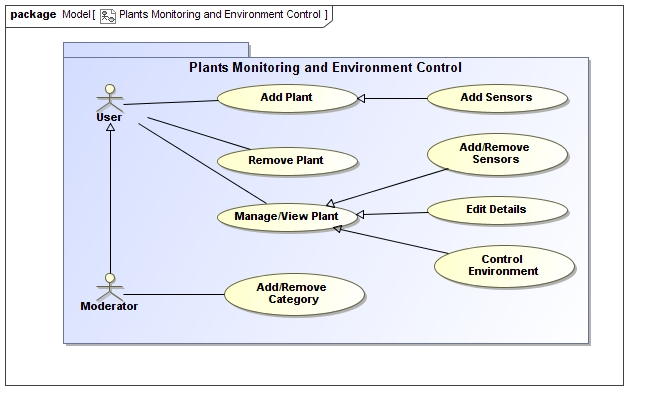
\includegraphics[width=\textwidth]{Plants_Monitoring_and_Environment_Control.jpg}
			\caption{The scope of functionality required from the \emph{Plants Monitoring and Environment Control} module}
		\end{figure}
		
		The scope of the \emph{Plants Monitoring and Environment Control} module includes:
		
		\begin{itemize}
			\item Adding a plant, which includes adding sensors to the plant object.
			\item Removing plants from the system, which will remove the plant object from the current plant view, but not from the database.
			\item Managing and viewing current plants' details and settings, which includes adding and removing sensors, editing plant details and changing the environment control parameters.
			\item Adding and removing categories of plants, which can only be done by a moderator.
		\end{itemize}
		
	\pagebreak
	\subsection{People}
		The scope of the \emph{People} module is shown below in Figure 2.
		
		\begin{figure}[H]
			\centering
			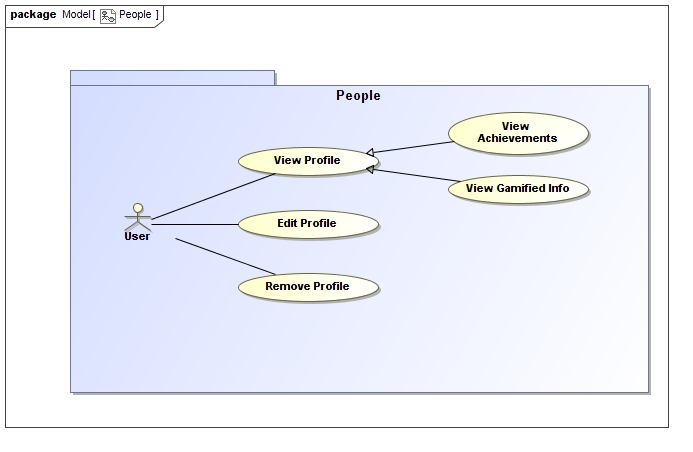
\includegraphics[width=\textwidth]{People.jpg}
			\caption{The scope of functionality required from the \emph{People} module}
		\end{figure}
		
		The scope of the \emph{People} module includes:
		
		\begin{itemize}
			\item Letting a user view their profile, on which will be achievements and gamified information (like badges and progress).
			\item Allowing a user to edit their profile information.
			\item Deleting of profiles.
		\end{itemize}
		
	\pagebreak
	\subsection{Analytics}
		The scope of the \emph{Analytics} module is shown below in Figure 3.
		
		\begin{figure}[H]
			\centering
			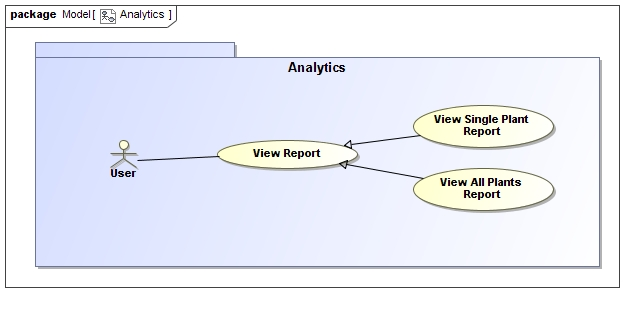
\includegraphics[width=\textwidth]{Analytics.jpg}
			\caption{The scope of functionality required from the \emph{Analytics} module}
		\end{figure}
		
		The scope of the \emph{} module includes:
		
		\begin{itemize}
			\item Viewing reports of either a single plant or a summary of all plant details.
		\end{itemize}
		
	\pagebreak
	\subsection{Notifications}
		The scope of the \emph{Notifications} module is shown below in Figure 4.
		
		\begin{figure}[H]
			\centering
			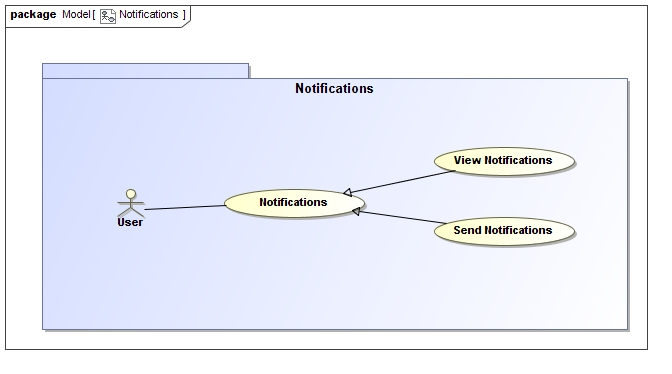
\includegraphics[width=\textwidth]{Notifications.jpg}
			\caption{The scope of functionality required from the \emph{Notifications} module}
		\end{figure}
		
		The scope of the \emph{} module includes:
		
		\begin{itemize}
			\item Viewing recieved notifications.
			\item Sending notifications to other users.
		\end{itemize}

\cleardoublepage

\section{Architectural Requirements}
\subsection{Access and Integration Requirements}
The system will be accessed by the users through a web browser. This could be from a mobile device or a computer. 
\begin{itemize}
	\item The IoT devices integrate with MQTT through the hardware API to queue and send events to AWS Lambda, where the data will be processed and persisted to DynamoDB
	\item The web interface will integrate with the AWS API Gateway's REST interface in order to send requests to Lambda. Lambda will then perform the necessary actions, access the database if needed and then return relevant information if required
\end{itemize} 
\subsection{Quality Requirements}

\subsubsection{Maintainability}
The system should be designed and created in such a way that it easy to maintain in the future.
\begin{itemize}
	\item New developers should be able to easily understand the system
	\item It should be easy to modify parts of the system
	\item Adding new functionality should be easy and straightforward
	\item SDKs are available for all the Amazon Web Services which are constantly being maintained and documented allowing for other developers to easily understand the infrastructure of the project
\end{itemize}
\subsubsection{Flexibility}
It is important that the system has support for many hardware components such as sensors. These technologies are advancing rapidly, therefore it should be easy to add new components to the system, without making any large changes.

	\begin{itemize}
		\item Flexibility in terms of easily adding or removing resources and functions to API Gateway
		\item Easily add or remove Lambda functions
		\item The system should be able to function with any number of sensors, it is not imperative that a user has all the necessary sensors in order to use the system
	\end{itemize}
\subsubsection{Extensibility}
	\begin{itemize}
		\item The system should be able to have extra sensors added which it can then monitor
	\end{itemize}
\subsubsection{Performance}
	\begin{itemize}
		\item The UI should respond in less than 0.2 seconds excluding external influences out of the control of the system
		\item Lambda functions should executed within under 5 seconds
		\item Getting and setting information with regard to the database should be executed under 5 seconds
		\item Conditions of plants need to be monitored within real time and should be queued to be sent to the database. Every 20 minutes the hardware should trigger an event to send the information to Lambda or to DynamoDB. If there is no connection available the hardware should continue to queue data until a connection is established.
	\end{itemize}
\subsubsection{Scalability}
	\begin{itemize}
		\item System will be able to support 10 000 concurrent users and should be able to scale upwards to handle hundreds of thousands of concurrent calls
		\item The system will be able to support up to 2000 plant boxes and should be able to scale proportionally with regard to the number of users (Up to hundreds of thousands of concurrent calls)
	\end{itemize}
\subsubsection{Security}
	\begin{itemize}
		\item All personal user information should be kept private and should not be accessible by other users
		\item User authentication and authorization should be performed
		\item Passwords should be hashed and salted
		\item Personal information such as passwords should be encrypted when being sent over the network
	\end{itemize}
\subsubsection{Auditabilty}
	\begin{itemize}
		\item API Gateway should monitor performance metrics as well as information on API calls, data latency and error rates.
		\item Conditions of the environment of the plants should be monitored in real time
		\item Each sensor should be distinguishable from the others so as to track where the data originates from
		\item The logs of the sensors will be persisted within the database so that analytics can be performed on them
		\item The results of the sensor logs will be made available via the user interface to the users
		\item The system will not allow the audit log to be modified
	\end{itemize}
\subsubsection{Usability}
	\begin{itemize}
		\item The system should be intuitive and efficient to use
		\item Users with basic computer literacy should be able to easily use the core functionality of the system
		\item Error messages should be clear
		\item Input validation should be done on the client side as much as possible
	\end{itemize}
\subsubsection{Reliability}
	\begin{itemize}
		\item The system should not have a single point of failure
		\item The system should have a reasonable amount of availability
	\end{itemize}
\subsubsection{Testability}
	\begin{itemize}
		\item The system should support multiple versions of the same API, allowing for quick iterations, testing and releasing of new versions.
		\item The system should support mock objects for testing in place of hardware if none is available
		\item Tests should be run to ensure that a function is only called if all pre-conditions for said function have been met
		\item Tests should be run to ensure after a function has executed all post-conditions are true
		\item The system should be able to test other quality requirements where possible
	\end{itemize}
\subsubsection{Deployability}
	\begin{itemize}
		\item The system will be deployed through on Amazon Web Services such as Lambda and DynamoDB
		\item The system should be able to deploy multiple versions of the same API for testing
	\end{itemize}
\subsubsection{Cost}
	\begin{itemize}
		\item The system should only cost as much as the resources it is using at a particular instance
	\end{itemize}
\subsubsection{Integrability}
	\begin{itemize}
		\item The system should be able to integrate well between the Amazon Web Services which are being used
		\item Future integration requirements should be easily addressable by using widely adopted public standards
		\item The system should be able to integrate with different hardware as long as the hardware queues information using a standardized format using MQTT
	\end{itemize}

\subsection{Architectural Responsibilities}
The architectural responsibilities for the system as a whole are shown below
\begin{figure}[H]
	\centering
	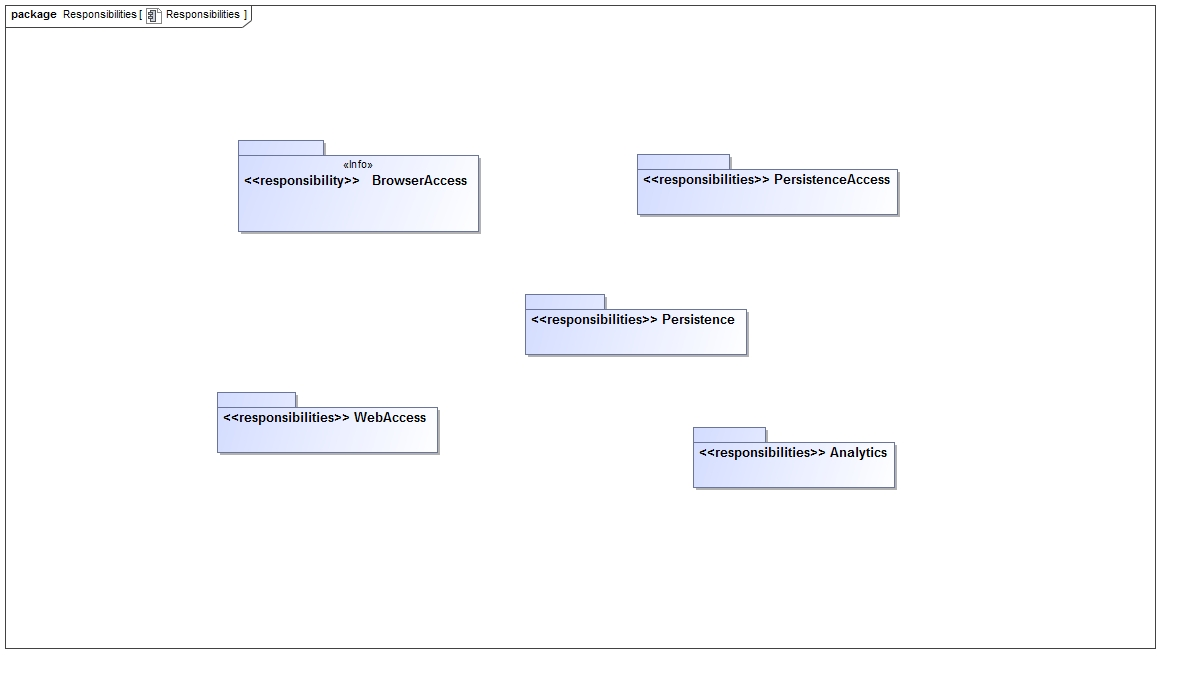
\includegraphics[width=\textwidth]{Responsibilities.jpg}
	\caption{Architectural responsibilities of the system}
\end{figure}
\clearpage
\subsection{Architecture Constraints}
\subsubsection{REST}
	REST has the following architectural constraints:
	\begin{itemize}
		\item Decouples consumers from producers
		\item Stateless existence
		\item Able to leverage a cache
		\item Leverages a layered system
		\item Leverages a uniform interface
	\end{itemize}

\cleardoublepage

\section{Architecture Design}
\subsection{Architectural Tactics}
	\subsubsection{Overall Software Architecture}
		\paragraph{Event-Driven Programming}\mbox{}\\
		The program flow will be determined by events. The user interface will make API calls via the use of RESTful services exposed by API Gateway. Lambda functions will only be called upon the triggering of events by the user via the user interface via API Gateway. DynamoDB will be able to receive data from Lambda after an event has been triggered as well as trigger its own events based on information which it receives. The IoT hardware platform will also be able to trigger events to call Lambda functions via the use of IoT Gateway.\\\\
		This paradigm ensures lower running costs as well as the creation of an almost autonomous system which reacts to events only when they occur. This tactic also allows for complex event processing whereby multiple events can be analysed to determine a larger picture.\\\\
		This provides scalability and performance quality attributes in terms of being able to increase processing power on demand to scale-up resources. It also enables the ease of managing resource demand through efficient processing which is only used when it is required as a way to reduce load.
	\subsubsection{API - Amazon API Gateway}
		\paragraph{REST}\mbox{}\\
		RESTful services will be exposed via the use of API Gateway. Our web application would then be able to call publicly available AWS services through code running in AWS Lambda.\\\\
		REST provides accessibility and integrability quality attributes through ensuring the goal of providing access. It does this through enforcing standard communication protocols.
		\paragraph{Monitoring \& Testing}\mbox{}\\
		Amazon API Gateway enables easy monitoring in terms of performance metrics and information on API calls, data latency and error rates. Using this information we will be able to ensure reliability and availability through the detection and recovering of faults. Amazon API Gateway also enables multiple different versions of the same API to be deployed so as to enable testing. Through the use of this we will be able to prevent faults so as to achieve a higher level of reliability.
	\subsubsection{Database - DynamoDB}
		\paragraph{Dynamo Storage}\mbox{}\\
		Dynamo refers to a set of techniques that when taken together can form a key-value structured storage system or a distributed data store. It combines properties of databases as well as distributed hash tables. Dynamo provides scalability and performance quality attributes through the managing of resource demand via spreading the load of the resources. Dynamo also enables the increasing of storage by scaling up resources.\\\\
		\textit{Principles of Dynamo Systems:}
		\begin{itemize}
			\item Incremental scalability
			\item Symmetry
			\item Decentralization
			\item Heterogeneity
		\end{itemize}
		The above principles aim to ensure that Dynamo is able to scale out each storage host (node) and that each node has the same set of responsibilities and therefore no nodes have special responsibilities. They also ensure that there is no central control and therefore no central point of failure. Dynamo ultimately also ensures that the work is distributed equally and that the distribution is proportional across all nodes according to the workload.
	\subsubsection{Backend Processing - Lambda}
		\paragraph{Lambda Functions}\mbox{}\\
		Lambda is the main driving force behind our event-driven design and consists of Lambda functions. These are always available to run as soon as they are triggered by some sort of event. They are stateless with no affinity to the underlying infrastructure so that Lambda can launch as many copies of the function as needed to scale for incoming events.
		
		Hence Lambda functions provide scalability and performance quality attributes as they ensure the ability to scale up resources via the increase of processing power.
	\subsubsection{Hardware - IoT Hardware Platform}
		\paragraph{MQTT}\mbox{}\\
		The hardware used will be gathering a lot of information in real time and therefore it is imperative that this information is queued. The reasoning behind using a queueing system is that queueing offers the following main benefits:
		\begin{itemize}
			\item There are no direct connections between programs - can easily mock out the queued data
			\item Pre-processing can be performed whilst the data is queued
			\item Communication between programs can be independent of time - this will help in the case of loss of connection to the hardware
			\item Communication can be driven by events
		\end{itemize}
		
		The above ensures that scalability and performance can be achieved through the managing of resource demand by spreading the load and using queueing. It also ensures more efficient processing by only using processing power when there is enough data to process hence effectively reducing the load on the machines.
	
\subsection{Infrastructure}
	We will be using the Amazon WebServices SDK and APIs as we need to use the AWS IoT (Internet of Things) platform for the project. As such, we will be using other AWS products together with IoT due to their seamless intergration.
		\begin{figure}[H]
			\centering
			\includegraphics[width=\textwidth]{AWSMap.png}
			\caption{Communication between AWS services}
		\end{figure}
	\subsubsection{Internet of Things}
		AWS IoT is a managed cloud platform that lets connected devices easily and securely interact with cloud applications and other devices.
		
		We will be using the IoT platform to connect to Lambda (explained below) using the MQTT protocol. As part of the project, we are required to use the AWS IoT platform.
	\subsubsection{Lambda}
		AWS Lambda lets us run code without provisioning or managing servers. You pay only for the compute time you consume - there is no charge when your code is not running. With Lambda, you can run code for virtually any type of application or backend service - all with zero administration. We can just upload our code and Lambda takes care of everything required to run and scale our code with high availability. We can set up your code to automatically trigger from other AWS services or call it directly from any web or mobile app.
		
		Lambda will form the largest part of our backend. All messages will be sent from IoT to Lambda, using MQTT, and that event will trigger a response and the web interface can access Lambda through the API Gateway, negating the need for a server to be constantly listening. Lambda can then perform operations on DynamoDB, but can also respond to events triggered when data in DynamoDB is changed or added. 
	\subsubsection{DynamoDB}
		Amazon DynamoDB is a fast and flexible NoSQL database service which has built in Java support. Because it is a NoSQL database, we can push and pull Java objects using the API. It intergrates with AWS Lambda, allowing Lambda to respond to events in the database. It can also be easily accessed through the API Gateway, allowing for fast read-write operations from the client interface.
	\subsubsection{API Gateway}
		Amazon API Gateway is a fully managed service that makes it easy for developers to create, publish, maintain, monitor, and secure APIs at any scale. We can easily and quickly create an API that acts as a “front door” for the user interface to access data from DynamoDB or trigger events in Lambda by exposing RESTful services to the API. Amazon API Gateway handles all the tasks involved in accepting and processing up to hundreds of thousands of concurrent API calls, including traffic management, authorization and access control, monitoring, and API version management.
	\subsubsection{JavaScript SDK}
		The AWS SDK for JavaScript enables us to directly access AWS services from JavaScript code running in the browser. We can authenticate users, store data in DynamoDB and trigger Lambda events. It is simple to deploy and uses the same API as the other components, meaning function migration becomes trivial.

\subsection{Concepts and Constraints for Application Components}
In terms of data persistence:
\begin{itemize}
	\item We will be using Java objects to store plant-based information with long-living state
	\item The state of these data objects will be modified and retrieved using DynamoDB.
\end{itemize}
These objects will store only data, and thus be devoid of any business processes.
\end{document}
